The InReport component encapsulates an incoming report in a user application. This component enforces the generic behaviour that is common to all incoming reports irrespective of their type and it provides read-only access to a report's attributes.

The InReport component is an extension of the Base Component of section \ref{sec:BaseCmp}. Incoming reports must be accepted before they can be executed (see section \ref{sec:RepLifecycle}). The acceptance check is implemented partly by the InLoader (see section \ref{sec:InLoader}) and partly by \chgC{the configuration} checks of the InReport itself.

\begin{figure}[h]
 \centering
 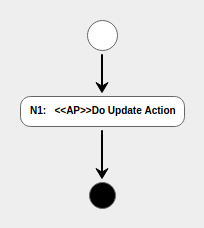
\includegraphics[scale=0.4,keepaspectratio=true]{InReportExecution.png}
 \caption{The InReport Execution Procedure}
 \label{fig:InReportExecution}
\end{figure}

The behaviour of a report that has been accepted is modelled by the procedure shown in figure \ref{fig:InReportExecution} (the \textit{InReport Execution Procedure}). This procedure is used as execution procedure for the InReport. The procedure simply executes the InReport's Update Action and then terminates. The Update Action is an adaptation point.

The InReport component provides visibility over all attributes of the reports it \chgC{encapsulates. The operation to set and get the} value of the report attributes is therefore an adaptation point for the InCommand.

